\documentclass[12pt]{article}

\usepackage{amssymb}
\usepackage{amsthm, amsmath}
\usepackage{graphicx}
\usepackage{natbib}
\usepackage{color}

\usepackage{tikz}
\usetikzlibrary{decorations.markings}
\usetikzlibrary{decorations.pathmorphing}

\newcommand{\solphys}{Solar Physics}

%\renewcommand{\thefootnote}{\fnsymbol{footnote}}


\title{Initial value problem of a finite beta asymmetric magnetic slab}
\date{}

\begin{document}
\maketitle

\section{TO DO}
\begin{itemize}
	\item Calculate residues for fast body modes.
	\item Check that there aren't any leaky modes on other Riemann sheets (I don't think there is because we have branch points from the square roots, not from logarithmic terms, so there are only two Riemann sheets).
	\item Try initial conditions.
\end{itemize}

\section{Basic equations}
From \cite{and_etal07},
\begin{equation}
\frac{1}{\rho(\omega^2 - \omega_A^2)} \left( \frac{\partial^2}{\partial x^2} - m^2 \right) \hat{p}_T = f(\omega, x),
\end{equation}
where
\begin{align}
f(\omega, x) &= \frac{\partial}{\partial x} \frac{\dot{\xi}_{x0} - i\omega\xi_{x0}}{\rho(\omega^2 - \omega_A^2)} + ik_y \frac{\dot{\xi}_{y0} - i\omega\xi_{y0}}{\rho(\omega^2 - \omega_A^2)} + ik_z \frac{c_0^2}{c_0^2 + v_A^2} \frac{\dot{\xi}_{z0} - i\omega\xi_{z0}}{\rho(\omega^2 - \omega_T^2)}, \\
m^2 &= m(\omega)^2 = \frac{(\omega_1^2 - \omega^2)(\omega_2^2 - \omega^2)}{(c_0^2 + v_A^2)(\omega_T^2 - \omega^2)}, \\
\omega_1^2 &= \frac{1}{2}(k_y^2 + k_z^2)(c_0^2 + v_A^2) \left( 1 - \sqrt{1 - \frac{4\omega_T^2}{(k_y^2 + k_z^2)(c_0^2 + v_A^2)}} \right), \\
\omega_2^2 &= \frac{1}{2}(k_y^2 + k_z^2)(c_0^2 + v_A^2) \left( 1 + \sqrt{1 - \frac{4\omega_T^2}{(k_y^2 + k_z^2)(c_0^2 + v_A^2)}} \right).
\end{align}

Take $k_y \ll k_z$ and $\xi_{y0} = \dot{\xi}_{y0} = 0$, then
\begin{equation}
\left( \frac{\partial^2}{\partial x^2} - m^2 \right) \hat{p}_T = f(\omega, x),
\end{equation}
where
\begin{align}
f(\omega, x) &= \frac{\partial}{\partial x} (\dot{\xi}_{x0} - i\omega\xi_{x0}) + ik_z \frac{c_0^2}{c_0^2 + v_A^2} \frac{(\omega^2 - \omega_A^2)}{(\omega^2 - \omega_T^2)} (\dot{\xi}_{z0} - i\omega\xi_{z0}), \\
m^2 &= \frac{(\omega_0^2 - \omega^2)(\omega_A^2 - \omega^2)}{(c_0^2 + v_A^2)(\omega_T^2 - \omega^2)},
\end{align}
where we have defined the initial values by
\begin{equation}
\xi_x(x, 0) = \xi_{x0}, \quad \frac{\partial{}\xi_x}{\partial{t}}(x, 0) = \dot{\xi}_{x0}, \quad \xi_z(x, 0) = \xi_{z0}, \quad \frac{\partial{}\xi_z}{\partial{t}}(x, 0) = \dot{\xi}_{z0}.
\end{equation}

Considering a magnetic slab in a non-magnetic environment, we have
\begin{align}
m_0^2 &= - \frac{(\omega^2 - \omega_0^2)(\omega^2 - \omega_A^2)}{(c_0^2 + v_A^2)(\omega^2 - \omega_T^2)}, \quad m_{1,2}^2 = \frac{\omega_{1,2}^2 - \omega^2}{c_{1,2}^2}, \\
f_{1,2}(\omega,x) &= \frac{\partial}{\partial x} (\dot{\xi}_{x0} - i\omega\xi_{x0}) + ik(\dot{\xi}_{z0} - i\omega\xi_{z0}).
\end{align}


\section{Solution in Laplace space}

\subsection{Solution within the slab}
For the solution inside the slab, $|x| < x_0$, $\hat{p}_T(x)$ satisfies
\begin{equation}
\left( \frac{\partial^2}{\partial x^2} - m_0^2 \right) \hat{p}_T = f_0(\omega, x),
\end{equation}
under the boundary conditions $\hat{p}_T(-x_0) = \hat{A}_1$ and $\hat{p}_T(-x_0) = \hat{A}_2$. To solve this we construct the Green's function, $G_0(x;s)$ that satisfies
\begin{equation}
\frac{d^2G_0}{dx^2} - m_0^2 G_0 = \delta(x-s), \quad G_0(-x_0;s) = G_0(x_0;s) = 0,
\end{equation}
where $\delta$ denotes the Dirac delta function. The general solution of this equation is
\begin{equation}
G_0(x;s) = c_1\sinh(m_0(x - x_0)) + c_2\sinh(m_0(x + x_0)),
\end{equation}
where $c_1 = 0$ for $x < s$ and $c_2 = 0$ for $x > s$. Ensuring $G_0$ and $\partial G_0 / \partial x$ have jumps of 0 and 1 at $x = s$, respectively, determines $c_1$ and $c_2$ so that $G_0(x;s)$ is
\begin{equation}
G_0(x;s) = \frac{-1}{m_0\sinh(2m_0 x_0)}
\begin{cases}
\sinh(m_0(x_0 - s))\sinh(m_0(x_0 + x)), & \text{if } -x_0<x<s, \\
\sinh(m_0(x_0 - x))\sinh(m_0(x_0 + s)), & \text{if } s<x<x_0.
\end{cases}
\end{equation}
Then the solution of Equation~\eqref{P eq inside} is
\begin{equation}
\hat{p}_T(x) = \frac{1}{m_0\sinh{2m_0 x_0}} \left[ \hat{A}_1\sinh(m_0(x_0 - x)) + \hat{A}_2\sinh(m_0(x_0 + x)) \right] + \int_{-x_0}^{x_0} G_0(x;s) f_0(\omega, s) ds.
\label{P sol 0}
\end{equation}
This is the sum of the Green's function term and a two terms that are independent solutions to the homogeneous version of Equation~\eqref{P eq inside} that ensure that the inhomogeneous boundary conditions are satisfied.


\subsection{Solution outside the slab}
For the solution outside and to the left of the slab, $x < -x_0$, $\hat{p}_T(x)$ satisfies
\begin{equation}
\left(\frac{d^2}{dx^2} - m_1^2 \right) \hat{p}_T = f_1(\omega, x),
\end{equation}
and the boundary conditions $\hat{p}_T(-\infty) = 0$, $\hat{p}_T(-x_0) = \hat{A}_1$. By following a Green's function method, the solution of this Sturm-Liouville system is
\begin{equation}
\hat{p}_T(x) = \hat{A}_1e^{m_1(x_0+x)} + \int_{-\infty}^{-x_0} G_1(x; s) f_1(\omega, s) ds,
\label{P sol 1}
\end{equation}
where $m_1 > 0$ and the Green's function, $G_1$, is defined by
\begin{equation}
G_1(x; s) = \frac{1}{m_1}
\begin{cases}
e^{m_1(x_0 + x)}\sinh(m_1(x_0 + s)), & \text{if } x < s, \\
e^{m_1(x_0 + s)}\sinh(m_1(x_0 + x)), & \text{if } s < x < -x_0.
\end{cases}
\end{equation}

Similarly, for the solution outside and to the right of the slab, $x > x_0$, $\hat{p}_T(x)$ satisfies
\begin{equation}
\hat{p}_T(x) = \hat{A}_2e^{m_2(x_0-x)} + \int_{x_0}^{\infty} G_2(x; s) f_2(\omega, s) ds,
\label{P sol 2}
\end{equation}
where $m_2 > 0$ and the Green's function, $G_2$, is defined by
\begin{equation}
G_2(x; s) = \frac{1}{m_2}
\begin{cases}
e^{m_2(x_0 - s)}\sinh(m_2(x_0 - x)), & \text{if } x_0 < x < s, \\
e^{m_2(x_0 - x)}\sinh(m_2(x_0 - s)), & \text{if } s < x.
\end{cases}
\end{equation}

Putting all of this together, the (Laplace transform of) total pressure is
\begin{equation}
\hat{p}_T(x) = 
\begin{cases}
\hat{A}_1e^{m_1(x_0 + x)} + \int_{-\infty}^{-x_0} G_1(x; s) f_1(\omega, s) ds, & \text{if } -\infty < x < -x_0, \\

\frac{1}{\sinh{2m_0x_0}} \left[ \hat{A}_1\sinh(m_0(x_0 - x)) + \hat{A}_2\sinh(m_0(x_0 + x)) \right] + \int_{-x_0}^{x_0} G_0(x; s) f_0(\omega, s) ds, & \text{if } -x_0 < x < x_0, \\

\hat{A}_2e^{m_2(x_0 - x)} + \int_{x_0}^{\infty} G_2(x; s) f_2(\omega, s) ds, & \text{if } x_0 < x < \infty.
\end{cases}
\label{P sol}
\end{equation}


\subsection{Matching solutions}
For physically relevant solutions, we require that the transverse displacement (equivalently, the perturbation in transverse velocity) and the total pressure be continuous across the interfaces at $x = \pm x_0$.

Continuity in total pressure perturbation, $\hat{p}_T$, is satisfied automatically by considering the solutions inside and outside the slab given by Equations~\eqref{P sol 0}, \eqref{P sol 1}, and~\eqref{P sol 2}, respectively, and our definition of $\hat{A}_1 = \hat{p}_T(-x_0)$ and $\hat{A}_2 = \hat{p}_T(x_0)$.

Continuity in transverse displacement, $\xi_x$, can be dealt with as follows. If we make the simplification to the prescribed initial conditions such that $\dot{\xi}_{x0} - i\omega\xi_{x0} = 0$, then this boundary condition is equivalent to
\begin{equation}
\left[ \left[ \frac{1}{\rho(\omega^2 - \omega_A^2)} \frac{\partial \hat{p}_T}{\partial x} \right] \right]_{x=\pm x_0} = 0.
\end{equation}
(Equation~(8) in \cite{and_etal07}).

Substituting the solutions given by Equations~\eqref{P sol 0}, \eqref{P sol 1}, and~\eqref{P sol 2} into these boundary conditions gives
\begin{equation}
\hat{A}_1(\omega) = \frac{T_1(\omega)}{D(\omega)}, \quad \hat{A}_2(\omega) = \frac{T_2(\omega)}{D(\omega)},
\end{equation}
where
\begin{align}
T_1(\omega) = T_1[f](\omega) & = -(\Lambda_2\cosh{2m_0 x_0} + \Lambda_0\sinh{2m_0 x_0})(\Lambda_1 I_0^- + \Lambda_0 I_1) - \Lambda_1(\Lambda_0 I_2 + \Lambda_2 I_0^+), \\
T_2(\omega) = T_2[f](\omega) & = -\Lambda_2(\Lambda_1 I_0^- + \Lambda_0 I_1) - (\Lambda_1\cosh{2m_0 x_0} + \Lambda_0\sinh{2m_0 x_0})(\Lambda_0 I_2 + \Lambda_2 I_0^+), \\
D(\omega) & = \Lambda_0(\Lambda_1 + \Lambda_2)\cosh(2m_0x_0) + (\Lambda_0^2 + \Lambda_1\Lambda_2)\sinh(2m_0x_0),
\label{D}
\end{align}
where $\Lambda_j = \rho_j (\omega^2 - \omega_{Aj}^2) /  m_j$, for $j = 0, 1, 2$, and
\begin{align}
I_0^\pm &= I_0^\pm[f] = \frac{1}{m_0} \int_{-x_0}^{x_0} \frac{\sinh(m_0(x_0 \pm s))}{\sinh(2m_0x_0)} f(\omega, s) ds, \\
I_1 &= I_1[f] = \frac{1}{m_1} \int_{-\infty}^{-x_0} e^{m_1(s + x_0)} f(\omega, s) ds,
\quad
I_2 = I_2[f] = \frac{1}{m_2} \int_{x_0}^\infty e^{m_2(x_0 - s)} f(\omega, s) ds,
\end{align}
where
\begin{equation}
f(\omega, x) = \begin{cases}
f_1(\omega, x), &\text{if } x < -x_0, \\
f_0(\omega, x), &\text{if } -x_0 < x < x_0, \\
f_2(\omega, x), &\text{if } x_0 < x.
\end{cases}
\end{equation}


\section{Solution in time}
To recover the transverse velocity, $v_x(x, t)$, we employ the inverse Laplace transform (non-standard, discussed in Appendix~\ref{app: laplace trans}), such that
\begin{equation}
p_T(x,t) = \mathcal{L}^{-1}\{\hat{p}_T(x)\} = \frac{1}{2\pi} \lim_{L \to \infty} \int_{i\gamma - L}^{i\gamma + L} \hat{p}_T(x) e^{-i\omega t} d\omega,
\label{laplace transform}
\end{equation}
where $\gamma$ is a real number such that all the singularities of the integrand are below the contour of integration to ensure that all singularities contribute to the integral. The integral is evaluated along an infinite horizontal line in the upper half of the complex plane and is dependent on the singularities (with respect to $\omega$) of $\hat{p}_T$, whose residues determine the value of the contour integral.

Focusing firstly on the region $x < -x_0$, the solution is
\newcommand{\e}{\epsilon}
\begin{align}
p_T(x, t) &= \mathcal{L}^{-1} \left\{ \hat{A}_1 e^{m_1(x + x_0)} + \int_{-\infty}^{-x_0} G_1(x; s)f_1(\omega, s)ds \right\}, \\
&= \mathcal{L}^{-1} \left\{ \hat{A}_1 e^{m_1(x + x_0)} \right\} + \mathcal{L}^{-1} \left\{ \int_{-\infty}^{-x_0} G_1(x; s)f_1(\omega, s)ds \right\}.
\end{align}


\subsection{Asymptotic solution for large time}
To study the asymptotic behaviours of the total pressure perturbation, we start with the asymptotic behaviours of $A_1(t) = p_T(-x_0, t)$ and $A_2(t) = p_T(x_0, t)$. These variables can be determined, using the inverse Laplace transform (non-standard, discussed in Appendix~\ref{app: laplace trans}), to be
\begin{equation}
A_1(t) = \frac{1}{2\pi} \lim_{L \to \infty} \int_{i\gamma - L}^{i\gamma + L} \frac{T_1(\omega)}{D(\omega)} e^{-i\omega t} d\omega, \quad A_2(t) = \frac{1}{2\pi} \lim_{L \to \infty} \int_{i\gamma - L}^{i\gamma + L} \frac{T_2(\omega)}{D(\omega)} e^{-i\omega t} d\omega,
\label{A inv laplace}
\end{equation}
where $\gamma$ is a real number such that all the singularities of the integrands are below the contour of integration. The integrals are evaluated along an infinite horizontal line in the upper half of the complex plane.

Since the problem of finding the solution is now reduced to solving a complex integral, it is dependent on the singularities (with respect to $\omega$) of $T_1$, $T_2$, and $D$ (so that we can construct a Bromwich contour such that it is confined to a single-valued branch) and the zeros of $D$ (whose residues determine the value of the contour integral).

To determine the singularities of these functions, we determine the singularities of the constituent functions, as follows.
\begin{itemize}
	\item The functions $\Lambda_j^2$ are rational functions of $\omega$ with simple poles at $\omega = \pm \omega_{0j}$, for $j = 0, 1, 2$.
	
	\item $\Lambda_j$, for $j = 0, 1, 2$, involve radicals and have (algebraic) branch points at $\omega = \pm \omega_{Aj}$, $\pm \omega_{0j}$, and $\pm \omega_{Tj}$, respectively.\footnote{More precisely, $\omega = \pm \omega_{Aj}$, $\pm \omega_{0j}$, and $\pm \omega_{Tj}$ are the ramification points corresponding to the branch points $\Lambda_j(\omega)$, each with ramification index 2. However, the language used in the main text is common shorthand that is considered synonymous.}
	
	\item The functions $\cosh(z)$ and $\sinh(z)$ are entire functions of $z$ with only even and odd terms in their respective series expansions. Therefore, $\cosh(z)$ and $z\sinh(z)$ are entire functions of $z^2$. Hence, $\cosh(2m_0x_0)$ and $\Lambda_0\sinh{2m_0x_0}$ have only simple poles at $\omega = \omega_{T0}$.
	
	\item The integrands of $I_0^\pm$ are integrated with respect to $s$. Therefore, the singularities of $I_{1,2}$ are precisely the singularities of the integrands. The function $g(z) = \sinh(az) / \sinh(bz)$, for constants $a$ and $b \neq 0$ are entire functions of $z$, containing only even powers (once $g$ has been redefined as to remove the removable singularity at $z = 0$). Therefore, for another complex function $h$, the singularities of the composition $g \cdot h$ are precisely the singularities of the function $h(z^2)$. Hence, by letting $h(\omega) = m_0$, $a = s \pm x_0$, and $b = 2x_0$, it follows that $\sinh(m_0(s - x_0)) / \sinh(2m_0x_0)$ has simple poles at $\omega = \pm \omega_{T0}$.
	
	\item To determine the singularities of $I_{1,2}$, we need consider the singularities of the integrands. The functions $e^{a\sqrt{z}}$ and $e^{\frac{a}{\sqrt{z}}}$, for constant $a \neq 0$ have branch points at $z = 0$ that are algebraic (of ramification index 2) and transcendental, respectively. Therefore, by setting $a = x_0 \pm s$, it follows that the functions $e^{m_j(x_0 \pm s)}$, and therefore $I_j$, have algebraic branch points at $\omega = \pm \omega_{Aj}$ and $\pm \omega_{0j}$ and transcendental branch points at $\pm \omega_{Tj}$.
\end{itemize}
By the algebra of branch points, the set of branch points of a sum of functions is the union of the branch points of the constituent functions. Therefore, the branch points of both $T_1$ and $T_2$ are $\omega = \pm \omega_{A0,1,2}$ (algebraic), $\pm \omega_{00,1,2}$ (algebraic), $\pm \omega_{T0}$ (algebraic), and $\pm \omega_{T1,2}$ (transcendental). The dispersion function $D$ has branch points at $\omega = \pm \omega_{A0,1,2}$, $\pm \omega_{00,1,2}$, and $\pm \omega_{T0,1,2}$, all of which are algebraic.

\textcolor{red}{TO DO: Redo the above to show that we have algebraic branch points at all of the $\omega_{A,0,T}$ corresponding to the Alfven, slow and fast continua, corresponding to leaky modes. So we have 18 branch points. How should be choose the branch cuts? We need to ensure we are confined to a single Riemann sheet i.e. single valued. See e.g. Fig 6 in Sedlacek 1970.}

\textit{The above analysis determines that the singularities of each function $T_1(\omega)$, $T_2(\omega)$, and $D(\omega)$ are precisely the algebraic branch points at $\omega = \pm kv_{A1}$ and $\omega = \pm kv_{A2}$.}

\subsection{Asymptotic solution - non-magnetic external plasma}
If the external plasma is non-magnetic, \textit{i.e.} $v_{A1} = v_{A2} = 0$, then the integral has (algebraic) branch points at $\omega = \pm \omega_{A0}$, $\pm \omega_{00,1,2}$, and $\pm \omega_{T0}$, where, without loss of generality, we let $\omega_1 < \omega_2$. The contour, $C = C_1 + C_2 + C_3 + C_4 + C_5$ for the inverse Laplace transform can be modified as shown in Figure~\ref{fig: brom contour}. To ensure that the contour remains on a single Riemann surface, it is modified around the branch cuts so as to encircle the poles. The closed contour $C$ is a sum of the following sub-contours:
\begin{itemize}
	\item $C_0$: the horizontal line with imaginary part $\gamma$.
	\item $C_1$: the horizontal line from $L + \delta i$ to $\omega_0 + \delta i$, round the semicircle of radius $\delta$ and back along the horizontal line from $\omega_0 - \delta i$ to $L - \delta i$.
	\item $C_2$: the vertical lines from $\pm L + \gamma i$ to $\pm L + \delta i$ and the arcs of the large semicircle centred at the origin with radius $\Delta$.
	\item $C_3$: the vertical line up to, around, and back down from $\omega_T$.
	\item $C_4$: the vertical line up to, around, and back down from $-\omega_T$.
	\item $C_5$: the horizontal line from $-L - \delta i$ to $-\omega_0 - \delta i$, round the semicircle of radius $\delta$ and back along the horizontal line from $-\omega_0 + \delta i$ to $-L + \delta i$.
\end{itemize}
We use the integral along $C$ as $\delta \to 0$ and $L \to \infty$ to determine the inverse Laplace transform from Equation~\eqref{A inv laplace}. In the limit of $L \to \infty$, the integral along $C_0$ is identical to the desired integral in Equation~\eqref{A inv laplace}. The integrals along each of the sub-contours $C_1 - C_5$ are calculated in the following subsections.

\begin{figure}
	\centering
	\scalebox{0.9}{
		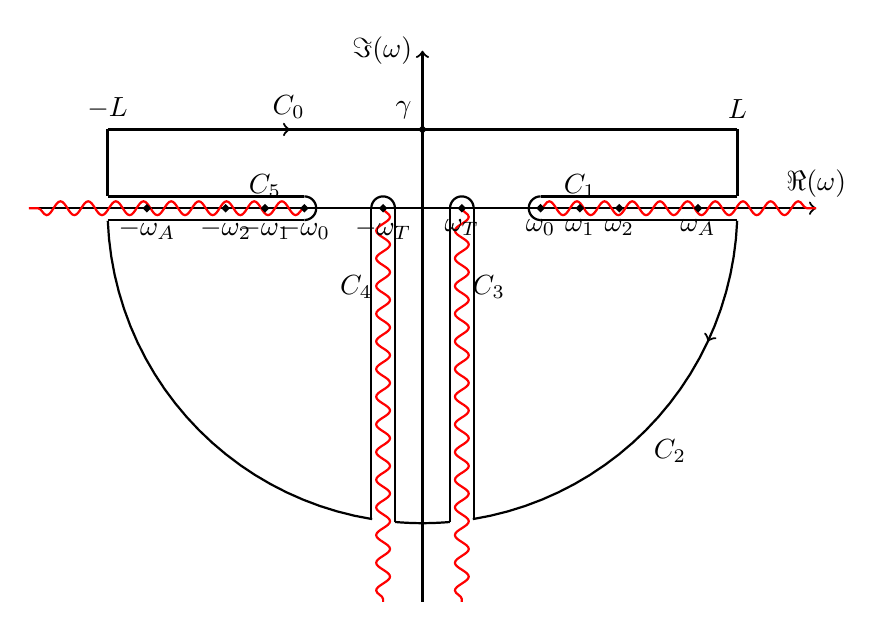
\begin{tikzpicture}[very thick, decoration={
			markings,
			mark=at position 0.29 with {\arrow{>}}}
		]
		
		\tikzset{
			branchcut/.style={decorate, decoration={snake}, draw=red}, 
		}
		
		\draw [->, thick] (-5,0) -- (5,0) node[above]{$\Re(\omega)$};
		\draw [->, thick] (0,-5) -- (0,2) node[left]{$\Im(\omega)$};
		
		\draw [postaction={decorate}, thick] (-4,1) -- (4,1);
		\draw [thick] (-4,1) -- (-4,0.15);
		\draw [thick] (4,1) -- (4,0.15);
		\draw [thick] (-4,0.15) -- (-1.5,0.15);
		\draw [thick] (4,0.15) -- (1.5,0.15);
		\draw [thick] (-4,-0.15) -- (-1.5,-0.15);
		\draw [thick] (4,-0.15) -- (1.5,-0.15);
		
		\draw [branchcut, thick] (0.5, 0) -- (0.5, -5);
		\draw [branchcut, thick] (-0.5, 0) -- (-0.5, -5);
		\draw [branchcut, thick] (1.5, 0) -- (5, 0);
		\draw [branchcut, thick] (-1.5, 0) -- (-5, 0);
		
		\draw [thick,domain=90:-90] plot ({0.15*cos(\x) - 1.5}, {0.15*sin(\x)});
		\draw [thick,domain=90:270] plot ({0.15*cos(\x) + 1.5}, {0.15*sin(\x)});
		
		\draw [postaction={decorate}, thick,domain=-2.3:-80.8] plot ({4*cos(\x)}, {4*sin(\x)});
		\draw [thick,domain=-85:-95] plot ({4*cos(\x)}, {4*sin(\x)});
		\draw [thick,domain=182.3:260.8] plot ({4*cos(\x)}, {4*sin(\x)});
		
		\draw [thick] (-0.35,0) -- (-0.35,-3.99);
		\draw [thick] (0.35,0) -- (0.35,-3.99);
		
		\draw [thick] (-0.65,0) -- (-0.65,-3.94);
		\draw [thick] (0.65,0) -- (0.65,-3.94);
		
		\draw [thick,domain=180:0] plot ({0.15*cos(\x) - 0.5}, {0.15*sin(\x)});
		\draw [thick,domain=180:0] plot ({0.15*cos(\x) + 0.5}, {0.15*sin(\x)});
		
		\node [above left] at (0,1) {$\gamma$};
		
		\draw[fill] (0,1) circle [radius=0.025];
		
		\draw[fill] (3.5,0) circle [radius=0.025];
		\node [below] at (3.5,0) {$\omega_{A}$};
		
		\draw[fill] (-3.5,0) circle [radius=0.025];
		\node [below] at (-3.5,0) {$-\omega_{A}$};
		
		\draw[fill] (2.5,0) circle [radius=0.025];
		\node [below] at (2.5,0) {$\omega_{2}$};
		
		\draw[fill] (-2.5,0) circle [radius=0.025];
		\node [below] at (-2.5,0) {$-\omega_{2}$};
		
		\draw[fill] (2,0) circle [radius=0.025];
		\node [below] at (2,0) {$\omega_{1}$};
		
		\draw[fill] (-2,0) circle [radius=0.025];
		\node [below] at (-2,0) {$-\omega_{1}$};
		
		\draw[fill] (1.5,0) circle [radius=0.025];
		\node [below] at (1.5,0) {$\omega_{0}$};
		
		\draw[fill] (-1.5,0) circle [radius=0.025];
		\node [below] at (-1.5,0) {$-\omega_{0}$};
		
		\draw[fill] (0.5,0) circle [radius=0.025];
		\node [below] at (0.5,0) {$\omega_{T}$};
		
		\draw[fill] (-0.5,0) circle [radius=0.025];
		\node [below] at (-0.5,0) {$-\omega_{T}$};
		
		\node [above] at (-1.7,1) {$C_0$};
		\node [above] at (2,0) {$C_1$};
		\node [below right] at (2.8,-2.8) {$C_2$};
		
		\node [right] at (0.5,-1) {$C_3$};
		\node [left] at (-0.5,-1) {$C_4$};
		\node [above] at (-2,0) {$C_5$};
		
		\node [above] at (4,1) {$L$};
		\node [above] at (-4,1) {$-L$};
		\end{tikzpicture} 
	}
	\caption{The Bromwich contour, $C = C_1 + C_2 + C_3 + C_4 + C_5$, for the complex integration of $\tilde{A}_{1,2}$ in the inverse Laplace transform in Equation~\eqref{A inv laplace}. The radius of the large semicircle is $L$ and the radius of the small semicircles around the points $\pm \omega_0$ and $\pm \omega_T$ is $\delta$.}
	\label{fig: brom contour}
\end{figure}


\subsubsection{Integral along $C_1$ and $C_5$}
In the limit as $\delta \to 0$, the integral along the semicircular part of $C_1$ approaches 0 because the integrand is analytic in this limit and the length of the contour approaches zero.

As $L \to \infty$ the integrals along $C_1$ become
\begin{align}
	I_{C_1} &= \int_{C_1} \frac{T_{1,2}}{D} e^{-i\omega t} d\omega \\
	&= \int_{\infty}^{\omega_0} \frac{T_{1,2}^+}{D^+} e^{-i\omega t} d\omega + \int_{\omega_0}^{\infty} \frac{T_{1,2}^-}{D^-} e^{-i\omega t} d\omega \\
	&= \int_{\omega_0}^{\infty} \left( \frac{T_{1,2}^-}{D^-} - \frac{T_{1,2}^+}{D^+} \right) e^{-i\omega t} d\omega,
\end{align}
where superscripts $+$ and $-$ indicate the value of the function above and below the horizontal branch cut $[\omega_0, \infty)$, respectively.

For values of $\omega$ between the branch points at $\omega_0$, $\omega_1$, $\omega_2$, and $\omega_A$, the integrand is analytic (except at the endpoints), therefore we can use integration by parts in these sub-intervals. For example, the integral over the sub-interval $(\omega_0, \omega_1)$ is
\begin{align}
I_{(\omega_0, \omega_1)} &= \int_{\omega_0}^{\omega_1} \left( \frac{T_{1,2}^-}{D^-} - \frac{T_{1,2}^+}{D^+} \right) e^{-i\omega t} d\omega \\
&= \frac{i}{t} \left\{ \left[ \left( \frac{T_{1,2}^-}{D^-} - \frac{T_{1,2}^+}{D^+} \right) e^{-i\omega t}\right]_{\omega_0}^{\omega_1} - \int_{\omega_0}^{\omega_1} \frac{d}{d\omega} \left( \frac{T_{1,2}^-}{D^-} - \frac{T_{1,2}^+}{D^+} \right) e^{-i\omega t} d\omega \right\}.
\end{align}
Given that $T_{1,2}^+(\omega_0)/D^\pm(\omega_0) = T_{1,2}^-(\omega_0)/D^\pm(\omega_0)$, the slowest decaying term is the first term on the right hand side evaluated at $\omega_1$, which decays like $\mathcal{O}(t^{-1})$ as $t \to \infty$. Repeating this for the other three intervals over which the integrand is analytic, and using the fact that $T_{1,2}^\pm(\omega)/D^\pm(\omega) \to 0$ as $|\omega| \to \infty$, we find that the slowest decaying terms decay like $\mathcal{O}(t^{-1})$$I_{C_1} = \mathcal{O}(t^{-1})$ as $t \to \infty$. Therefore $I_{C_1} = \mathcal{O}(t^{-1})$ (and similarly $I_{C_5} = \mathcal{O}(t^{-1})$) as $t \to \infty$.


\subsubsection{Integral along $C_2$}
As $L \to \infty$, points that occupy the curve $C_2$ will behave like $|\omega| \to \infty$. When $|\omega| \to \infty$, $T_{1,2} = \mathcal{O}(|\omega|)$ and $D = \mathcal{O}(|\omega|^2)$, therefore the integrands behave like $T_{1,2}/D = \mathcal{O}(1/|\omega|)$. Therefore the integral around $C_2$ approaches $0$ as $L \to \infty$.


\subsubsection{Integral along $C_3$ and $C_4$}
In the limit as $\delta \to 0$, the integral along the semicircular part of $C_3$ approaches 0 because the integrand is analytic in this limit and the length of the contour approaches zero. As $L \to \infty$ and $\delta \to 0$, the integrals along $C_3$ become
\begin{align}
I_{C_3} &= \int_{C_3} \frac{T_{1,2}}{D} e^{-i\omega t} d\omega \\
&= \int_{\omega_T}^{\omega_T - \infty i} \left( \frac{T_{1,2}^-}{D^-} - \frac{T_{1,2}^+}{D^+} \right) e^{-i\omega t} d\omega,
\end{align}
where superscripts $+$ and $-$ indicate the value of the function to the right and left of the vertical branch cut $\omega_T + [0,\infty)i$, respectively. The integrand is analytic in the integration interval (except at the endpoints), so by integration by parts
\begin{equation}
I_{C_3} = \frac{i}{t} \left\{ \left[ \left( \frac{T_{1,2}^-}{D^-} - \frac{T_{1,2}^+}{D^+} \right) e^{-i\omega t}\right]_{\omega_T}^{\omega_T -\infty i} - \int_{\omega_T}^{\omega_T - \infty i} \frac{d}{d\omega} \left( \frac{T_{1,2}^-}{D^-} - \frac{T_{1,2}^+}{D^+} \right) e^{-i\omega t} d\omega \right\}.
\end{equation}
the first term is zero because $T_{1,2}^\pm(\omega)/D^\pm(\omega) \to 0$ as $|\omega| \to \infty$ and $T_{1,2}^+(\omega_T)/D^\pm(\omega_T) = T_{1,2}^-(\omega_T)/D^\pm(\omega_T)$. Therefore, using integration by parts for a second time,
\begin{align}
I_{C_3} &= -\frac{i}{t} \int_{\omega_T}^{\omega_T - \infty i} \frac{d}{d\omega} \left( \frac{T_{1,2}^-}{D^-} - \frac{T_{1,2}^+}{D^+} \right) e^{-i\omega t} d\omega \\
&= \frac{1}{t^2} \left\{ \left[ \frac{d}{d\omega} \left( \frac{T_{1,2}^-}{D^-} - \frac{T_{1,2}^+}{D^+} \right) e^{-i\omega t}\right]_{\omega_T}^{\omega_T -\infty i} - \int_{\omega_T}^{\omega_T - \infty i} \frac{d^2}{d\omega^2} \left( \frac{T_{1,2}^-}{D^-} - \frac{T_{1,2}^+}{D^+} \right) e^{-i\omega t} d\omega \right\} \\
&= \mathcal{O}(t^{-2}) \text{ as } t \to \infty.
\end{align}
Similarly, $I_{C_5} = \mathcal{O}(t^{-2})$ as $t \to \infty$.


\subsubsection{Poles (AKA eigenfrequencies)}
Let $v_A > c_i$ for $i = 0, 1, 2$, then there can exist, in general:
\begin{enumerate}
	\item 2 slow surface modes,
	\item an infinite number of slow body modes,
	\item 2 fast surface modes.
\end{enumerate}
1 and 2 exist for all values of $kx_0$. 3 exist only for $kx_0$ values greater than a cut-off value. Analytical expressions for the behaviour of the eigenmodes do not exist in general. It is at this point that we are forced to make two simplifications to the model:
\begin{itemize}
	\item The thin-slab approximation, so that $kx_0 \ll 1$
	\item The approximate symmetry simplification, so that $\rho_1 \approx \rho_2$.
\end{itemize}
The eigenmodes of an asymmetric magnetic slab under these simplifications are given by the following expressions:
\begin{itemize}
	\item Slow quasi-sausage surface modes:
	\begin{equation}
		\omega^2=k^2c_\textrm{T}^2\left[1-\frac{2(kx_0)(c_0^2-c_\textrm{T}^2)}{(c_0^2+v_\textrm{A}^2)\left(\frac{\rho_0}{\rho_1}\frac{(c_1^2-c_\textrm{T}^2)^{1/2}}{c_1}+\frac{\rho_0}{\rho_2}\frac{(c_2^2-c_\textrm{T}^2)^{1/2}}{c_2}\right)}\right],
		\label{thinslab slow saus surf}
	\end{equation}
	which is less than $k^2c_\textrm{T}^2$ and exists only when $c_1>c_\textrm{T}$ and $c_2>c_\textrm{T}$.
	\item If $c_1=c_2=c_\textrm{e}$ (and therefore $\rho_1=\rho_2=\rho_\textrm{e}$), then there exists a fast sausage surface mode:
	\begin{equation}
		\omega^2=k^2c_\textrm{e}^2\left(1-\left[\frac{\rho_\textrm{e}}{\rho_0}\frac{c_\textrm{e}^2(c_0^2-c_\textrm{e}^2)(kx_0)}{(c_0^2+v_\textrm{A}^2)(c_\textrm{T}^2-c_\textrm{e}^2)}\right]^2\right)
		\label{thinslab fast saus surf}
	\end{equation}
	in the thin slab limit.
	\item Slow quasi-kink surface mode:
	\begin{equation}
		\omega^2=\frac{k^2x_0v_\textrm{A}^2\left(\frac{\rho_0}{\rho_1}m_1+\frac{\rho_0}{\rho_2}m_2\right)}{\left(\frac{\rho_0}{\rho_1}m_1x_0+\frac{\rho_0}{\rho_2}m_2x_0\right)+2}\approx{}\frac{1}{2}k^2v_\textrm{A}^2\left(\frac{\rho_0}{\rho_1}+\frac{\rho_0}{\rho_2}\right)kx_0.
		\label{thinslab slow kink surf}
	\end{equation}
	\item Quasi-sausage body solutions:
	\begin{equation}
		\omega^2=k^2c_\textrm{T}^2\left(1+\frac{c_\textrm{T}^4(kx_0)^2}{c_0^2v_\textrm{A}^2\pi^2j^2}\right), \quad j=1,2,\ldots. \label{thinslab saus body}
	\end{equation}
	\item Quasi-kink body solutions:
	\begin{equation}
		\omega^2=k^2c_\textrm{T}^2\left(1+\frac{c_\textrm{T}^4(kx_0)^2}{c_0^2v_\textrm{A}^2\pi^2(j-\frac{1}{2})^2}\right), \quad j=1,2,\ldots. \label{thinslab kink body}
	\end{equation}
\end{itemize}

Solution of the inverse Laplace transform is the sum of the residues at these points.

As shown in Appendix~\ref{app: approx sym DR}, under the approximate symmetry simplification, the dispersion function, $D(\omega)$, becomes
\begin{equation}
D(\omega) = \frac{\sinh{2m_0x_0}}{4\Lambda_1\Lambda_2} D_k(\omega) D_s(\omega),
\end{equation}
where
\begin{align}
D_k(\omega) &= \Lambda_0 (\Lambda_1 + \Lambda_2) + 2\Lambda_1\Lambda_2\coth(m_0x_0), \\
D_s(\omega) &= \Lambda_0(\Lambda_1 + \Lambda_2) + 2\Lambda_1\Lambda_2\tanh(m_0x_0).
\end{align}
This can be further simplified for surface modes under the thin-slab approximation, to first order in $kx_0$, to
\begin{align}
D_k(\omega) &= \Lambda_0 (\Lambda_1 + \Lambda_2) + 2\Lambda_1\Lambda_2\frac{1}{m_0x_0}, \\
D_s(\omega) &= \Lambda_0(\Lambda_1 + \Lambda_2) + 2\Lambda_1\Lambda_2m_0x_0.
\end{align}


\subsubsection{Residues}
In order to calculate the residue of each pole, we much determine their order. Firstly, for the slow kink surface mode, $\omega = \omega_{sks}$, it can be shown that $D_s(\omega_{sks}) \neq 0$, and after some algebra,
\begin{equation}
D_k(\omega) = \frac{\rho_1\rho_2\omega^2R}{m_0m_1m_2x_0} (\omega^2 - \omega_{sks}^2),
\end{equation}
where
\begin{equation}
R = 2 + \left( \frac{\rho_0}{\rho_1} + \frac{\rho_0}{\rho_2} \right)kx_0,
\end{equation}
so each of $\omega = \pm \omega_{sks}$ are simple zeros of $D_k$ and hence of $D$, therefore, they are simple poles of the integrand in question.

Therefore, the residue of the integrand at $\omega = \omega_{sks}$ is
\begin{align}
\mathrm{Res}\left\{ \frac{T_1}{D}e^{-i\omega t}; \omega = \omega_{sks} \right\} &= \lim_{\omega \to \omega_{sks}} \left\{ (\omega - \omega_{sks}) \frac{T_1(\omega)}{D(\omega)} e^{-i\omega t} \right\} \\
&= \frac{2m_0m_1m_2x_0\Lambda_1\Lambda_2}{\rho_1\rho_2\omega_{sks}^2Rm_0x_0}|_{\omega = \omega_{sks}} \frac{T_1(\omega_{sks})}{2\omega_{sks}D_s(\omega_{sks})} e^{-i\omega_{sks}t} \\
&= \frac{\omega_{sks}}{R} \frac{T_1(\omega_{sks})}{D_s(\omega_{sks})} e^{-i\omega_{sks}t}.
\end{align}
Similarly, the residue at $\omega = -\omega_{sks}$ is
\begin{equation}
\mathrm{Res}\left\{ \frac{T_1}{D}e^{-i\omega t}; \omega = -\omega_{sks} \right\} = \frac{\omega_{sks}}{R} \frac{T_1(\omega_{sks})}{D_s(\omega_{sks})} e^{i\omega_{sks}t}
\end{equation}
since $T_1$ and $D_s$ are even functions of $\omega$. 

Similarly, the residues for the slow sausage surface mode $\omega = \pm \omega_{sss}$ are 
\begin{align}
\mathrm{Res}\left\{ \frac{T_1}{D}e^{-i\omega t}; \omega = \omega_{sss} \right\} &= \lim_{\omega \to \omega_{sss}} \left\{ (\omega - \omega_{sss}) \frac{T_1(\omega)}{D(\omega)} e^{-i\omega t} \right\} \\
&= \frac{2m_0m_1m_2\Lambda_1\Lambda_2}{\rho_1\rho_2\omega_{sss}^2m_0x_0}|_{\omega = \omega_{sss}} \frac{(\omega_{sss}^2 - \omega_T^2)}{(\omega_{sss}^2 - \omega_A^2)k(\frac{\rho_0}{\rho_1}\sqrt{1 - \frac{c_T^2}{c_1^2}} + \frac{\rho_0}{\rho_2}\sqrt{1 - \frac{c_T^2}{c_2^2}})}\frac{T_1(\omega_{sss})}{2\omega_{sss}D_k(\omega_{sss})} e^{-i\omega_{sss}t} \\
&= \frac{\omega_{sss}}{kx_0} \frac{(\omega_{sss}^2 - \omega_T^2)}{(\omega_{sss}^2 - \omega_A^2)(\frac{\rho_0}{\rho_1}\sqrt{1 - \frac{c_T^2}{c_1^2}} + \frac{\rho_0}{\rho_2}\sqrt{1 - \frac{c_T^2}{c_2^2}})}\frac{T_1(\omega_{sss})}{D_k(\omega_{sss})} e^{-i\omega_{sss}t}.
\end{align}
Similarly, the residue at $\omega = -\omega_{sss}$ is
\begin{equation}
\mathrm{Res}\left\{ \frac{T_1}{D}e^{-i\omega t}; \omega = -\omega_{sss} \right\} = \frac{\omega_{sss}}{kx_0} \frac{(\omega_{sss}^2 - \omega_T^2)}{(\omega_{sss}^2 - \omega_A^2)(\frac{\rho_0}{\rho_1}\sqrt{1 - \frac{c_T^2}{c_1^2}} + \frac{\rho_0}{\rho_2}\sqrt{1 - \frac{c_T^2}{c_2^2}})}\frac{T_1(\omega_{sss})}{D_k(\omega_{sss})} e^{i\omega_{sss}t}.
\end{equation}

Regarding the fast kink body modes $\omega = \pm \omega_{fkbj}$, for $j = 1, 2, ...$, it can be shown that $|\cosh(m_0x_0)D_s(\omega_{fkbn})| \neq 0, \infty$. By letting $\omega_{fkbj}^2 = \omega_T^2(1 + v(kx_0)^2)$, for $v > 0$, we can show that\footnote{We consider the functions $D_s$ and $D_k$ multiplied by factors of $\cosh(m_0x_0)$ and $\sinh(m_0x_0)$, respectively, to ensure that singularities are regularised. The factors come from the $\sinh(2m_0x_0) = 2\sinh(m_0x_0)\cosh(m_0x_0)$ in the dispersion function $D$.}
\begin{align}
D(\omega(v)) &= \frac{\sinh(2m_0x_0)}{4\Lambda_1\Lambda_2}D_k(\omega(v))D_s(\omega(v)) \\
&= \frac{1}{2}\cosh(m_0x_0)D_s(\omega(v))\left[\cos\left(\frac{c_T}{\sqrt{(c_0^2 + v_A^2)v}}\right) + \mathcal{O}(kx_0)\right] \\
&= \frac{1}{2}\cosh(m_0x_0)D_s(\omega(v))\left[\frac{\pi(j + \frac{1}{2})(-1)^{j + 1}}{2\nu_j}(v - \nu_j) + \mathcal{O}((v - \nu_j)^2) + \mathcal{O}(kx_0)\right],
\end{align}
where $\nu_j = c_T^4 / c_0^2v_A^2\pi^2(j - \frac{1}{2})^2$ for $j \in \mathbb{N}$ such that $\omega_{fkbj} = \pm \omega_T\sqrt{1 + \nu_j(kx_0)^2}$ are simple zeros of the dispersion function $D$. Since $T_{1,2}(\omega_{fkbj}) \neq 0$, they are also simple poles of $T_{1,2}/D$. Therefore, the residues at $\omega = \omega_{fkbj}$ are\footnote{The zero of $\cosh(m_0x_0)$ when $\omega = \omega_{fkbj}$ regularises the singularities of $D_s(\omega)$.}
\begin{align}
\mathrm{Res}\left\{ \frac{T_1}{D}e^{-i\omega t}; \omega = \omega_{fkbj} \right\} &= \lim_{\omega \to \omega_{fkbj}} \left\{ (\omega - \omega_{fkbj}) \frac{T_1(\omega)}{D(\omega)} e^{-i\omega t} \right\} \\
&= \lim_{v \to \nu_j} \left\{ \frac{1}{2} \omega_T (kx_0)^2(v - \nu_j) \frac{T_1(\omega(v))}{D(\omega(v))} e^{-i\omega(v)t} \right\} \\
&= \frac{2(-1)^{j+1}\omega_T\nu_j(kx_0)^2}{\pi(j-\frac{1}{2})\cosh(m_0x_0)} \frac{T_1(\omega_{fkbj})}{D_s(\omega_{fkbj})}e^{-i\omega_{fkbj}t}.
\end{align}
Similarly, the residue at $\omega = -\omega_{fkbj}$ is
\begin{equation}
\mathrm{Res}\left\{ \frac{T_1}{D}e^{-i\omega t}; \omega = -\omega_{fkbj} \right\} = \frac{2(-1)^{j}\omega_T\nu_j(kx_0)^2}{\pi(j-\frac{1}{2})\cosh(m_0x_0)} \frac{T_1(\omega_{fkbj})}{D_s(\omega_{fkbj})}e^{i\omega_{fkbj}t}
\end{equation}

The residues for the fast sausage body modes, $\omega_{fsbj} = \pm \omega_T\sqrt{1 + \eta_j(kx_0)^2}$, where $\eta_j = c_T^4 / c_0^2v_A^2\pi^2j^2$ for $j \in \mathbb{N}$, are similarly given by
\begin{equation}
\mathrm{Res}\left\{ \frac{T_1}{D}e^{-i\omega t}; \omega = \omega_{fsbj} \right\} = \frac{2i(-1)^{j}\omega_T\eta_j(kx_0)^2}{\pi j\sinh(m_0x_0)} \frac{T_1(\omega_{fsbj})}{D_k(\omega_{fsbj})}e^{-i\omega_{fsbj}t}
\end{equation}
and
\begin{equation}
\mathrm{Res}\left\{ \frac{T_1}{D}e^{-i\omega t}; \omega = -\omega_{fsbj} \right\} = \frac{2i(-1)^{j}\omega_T\eta_j(kx_0)^2}{\pi j\sinh(m_0x_0)} \frac{T_1(\omega_{fsbj})}{D_k(\omega_{fsbj})}e^{i\omega_{fsbj}t}
\end{equation}

The residues for the integrand of $A_2$ are found by replacing subscript 2 with 1.



\appendix

\section{Non-standard Laplace transform}\label{app: laplace trans}
Consider a function $f(t)$, whose standard Laplace transform, $F_1(\omega)$, and non-standard Laplace transform, $F_2(\omega)$, are
\begin{equation}
F_1(\omega) = \int_0^\infty f(t) e^{-\omega t} dt,
\quad \text{and} \quad
F_2(\omega) = \int_0^\infty f(t) e^{i\omega t} dt.
\end{equation}
Trivially, $F_1(-i\omega) = F_2(\omega)$. Using the standard inverse Laplace transform, and letting $\gamma$ be real and greater than the real part of all the singularities of $F_1(\omega)$, the original function $f(t)$ can be written
\begin{align}
f(t) & = \frac{1}{2\pi i} \lim_{T\to\infty} \int_{\gamma - iT}^{\gamma + iT} F_1(\omega)e^{\omega t} d\omega, \\
& = \frac{1}{2\pi i} \lim_{T\to\infty} \int_{i\gamma - T}^{i\gamma + T} F_1(-i\omega)e^{-i\omega t} (-id\omega), \\
& = \frac{1}{2\pi} \lim_{T\to\infty} \int_{i\gamma - T}^{i\gamma + T} F_2(\omega)e^{-i\omega t} d\omega.
\end{align}
Therefore, the inverse transform of the non-standard Laplace transform is
\begin{equation}
f(t) = \frac{1}{2\pi} \lim_{T\to\infty} \int_{i\gamma - T}^{i\gamma + T} F_2(\omega)e^{-i\omega t} d\omega.
\end{equation}


\section{Approximately symmetric slab dispersion relation}\label{app: approx sym DR}
Consider the product of the following functions
\begin{align}
D_k(\omega) &= \Lambda_0 (\Lambda_1 + \Lambda_2) + 2\Lambda_1\Lambda_2\coth{m_0x_0}, \\
D_s(\omega) &= \Lambda_0(\Lambda_1 + \Lambda_2) + 2\Lambda_1\Lambda_2\tanh{m_0x_0}.
\end{align}
\begin{align}
D_k(\omega) D_s(\omega) &= \left[ \Lambda_0 (\Lambda_1 + \Lambda_2) + 2\Lambda_1\Lambda_2\coth{m_0x_0} \right] \left[ \Lambda_0(\Lambda_1 + \Lambda_2) + 2\Lambda_1\Lambda_2\tanh{m_0x_0} \right] \\
&= \Lambda_0^2 (\Lambda_1 + \Lambda_2)^2 + 2\Lambda_0(\Lambda_1 + \Lambda_2)\Lambda_1\Lambda_2(\tanh{m_0x_0} + \coth{m_0x_0}) + 4\Lambda_1^2\Lambda_2^2 \\
&= \frac{4\Lambda_1\Lambda_2}{\sinh{2m_0x_0}} \left[ \Lambda_0(\Lambda_1 + \Lambda_2)\cosh{2m_0x_0} + (\Lambda_0^2F + \Lambda_1\Lambda_2)\sinh{2m_0x_0} \right],
\end{align}
where
\begin{equation}
F = \frac{(\Lambda_1 + \Lambda_2)^2}{4\Lambda_1\Lambda_2},
\end{equation}
which, when the conditions on each side of the slab are approximately symmetric, \textit{i.e.} $\Lambda_2 = \Lambda_1 (1 + \epsilon L)$, with $\epsilon \ll 1$ and $L \approx 1$, becomes
\begin{equation}
F = \frac{(2 + \epsilon L)^2}{4(1 + \epsilon L)} = 1 + \mathcal{O}(\epsilon^2).
\end{equation}
Therefore, 
\begin{align}
D(\omega) &= \Lambda_0(\Lambda_1 + \Lambda_2)\cosh(2m_0x_0) + (\Lambda_0^2 + \Lambda_1\Lambda_2)\sinh(2m_0x_0), \\
&= \frac{\sinh{2m_0x_0}}{4\Lambda_1\Lambda_2} D_k(\omega) D_s(\omega) + \mathcal{O}(\epsilon^2).
\end{align}


\section{Approximately symmetric slab parameter expansions}
For an approximately symmetric slab, that is, when $\rho_2 = \rho_1(1 + \epsilon)$ where $\epsilon \ll 1$, then the first order expansions in $\epsilon$ of other relevant parameters are given below.
\begin{itemize}
	\item $c_2^2 = c_1^2 \frac{\rho_1}{\rho_2} = c_1^2 \left(\frac{1}{1 + \epsilon}\right) \approx c_1^2 (1 - \epsilon).$
	
	\item $m_2 = \sqrt{k^2 - \frac{\omega^2}{c_2^2}} = \sqrt{k^2 - \frac{\omega^2}{c_1^2}(1 + \epsilon)} \approx m_1(1 - \frac{\omega^2}{2c_1^2m_1^2}\epsilon)$.
	
	\item $\Lambda_2 = \frac{\rho_2 \omega^2}{m_2} = \frac{\rho_1(1 + \epsilon) \omega^2}{m_1\left(1 - \frac{1}{2m_1^2}\epsilon\right)} \approx \frac{\rho_1(1 + \epsilon) \omega^2}{m_1}\left(1 + \frac{1}{2m_1^2}\epsilon\right) = \Lambda_1\left( 1 + \epsilon \left[ 1 + \frac{\omega^2}{2c_1^2m_1^2} \right] \right)$.
	
	\item $I_2 = \int_{x_0}^\infty e^{m_2(x_0 - s)} f(\omega, s) ds = \int_{-\infty}^{-x_0} e^{m_2(x_0 + s)} f(\omega, s) ds$, if $f(\omega, -x) = f(\omega, x)~\forall x \in (-\infty, -x_0)$. Therefore,
	\begin{align}
		I_2 & = \int_{-\infty}^{-x_0} e^{\epsilon m_1M(x_0 + s)} e^{m_1(x_0 + s)} f(\omega, s) ds, \text{ where } M = -\frac{\omega^2}{2c_1^2m_1^2}, \\
		& = I_1 + \epsilon m_1M \int_{-\infty}^{-x_0} (x_0 + s) e^{m_1(x_0 + s)} f(\omega, s) ds.
	\end{align}
	It doesn't seem that this simplifies into $I_1(1 + J\epsilon)$ without making $f$ less general.
	
\end{itemize}

\bibliographystyle{unsrt}
\bibliography{../Bibliography}

\end{document}
